
\FloatBarrier

\section{Колебательная с зоной нечувствительности в возвращающей силе} % _DEADVI_

\LinkRef{
  deadvi: ASAU-20, ISDMCI-2013
}

\begin{equation}
\ddot{x} + c_0 \dot{x} + a \cdot x + b \cdot \mathrm{db}(x,x_0) = u(t),
\label{atu:eq:deadvi}
\end{equation}

$ u(t) = U_0 \sin( \omega_{in} t ) $.

Идентифицируемый параметр:
$ x_0 \in [2;2.5] $ -- ширина зоны нечувствительности.

Остальные параметры:
$U_0 = 1.4$, $\omega_{in} = 1.4$, $c_0=0.1$, $a=-0.3$, $b=1.0$.


\begin{figure}[htb!]
\centerline{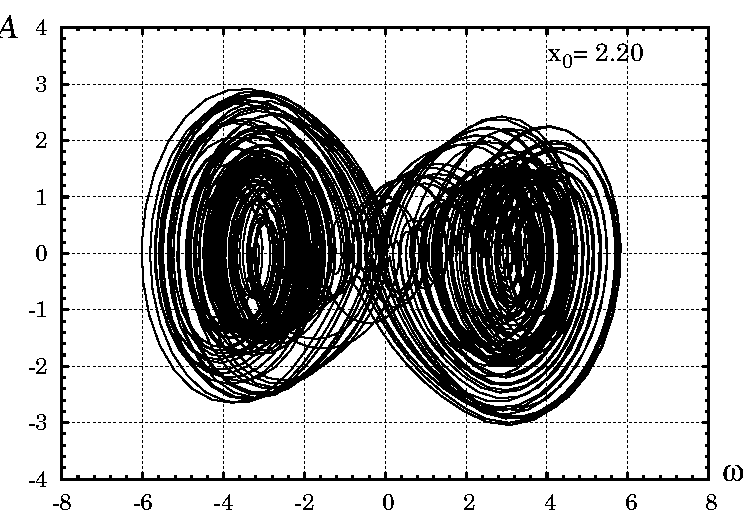
\includegraphics[width=0.5\textwidth]{p/cha/deadvi_phase.pdf} }
\caption{Фазовый портрет системы ``deadvi'' (\ref{atu:eq:deadvi})}
\label{atu:f:deadvi_phase}
\end{figure}

Критерий
$\overline{x^2(t)}$


